\begin{frame}{JRA-3Qとは？}{データ}
  \lead{気象庁の第 3 次長期再解析。$u, v, Z$ を 10 年ぶん使う \src{Kosaka+24}}
  \begin{cards}[3]
    \minicard{th-large}{0.375°}{約 40 km 格子}
    \minicard{layer-group}{38 面}{1000--3 hPa、約 0--40 km}
    \minicard{clock}{6 時間 × 10 年}{2016--2025、14,610 時刻}
  \end{cards}
  \vskip 1.5mm
  \begin{columns}[T]
    \begin{column}{0.72\textwidth}
      \begin{itemize}\itemsep 0.2mm
        \item \kw{なぜ JRA-3Q か}：国内の観測を厚く同化した気象庁製品
        \item 上端 0.01 hPa（約 80 km）。破裂高度を余裕で覆う
        \item 1947 年から現在まで。GDEX から無償 \src{JMA+24}
      \end{itemize}
    \end{column}
    \begin{column}{0.24\textwidth}
      \vskip -3mm
      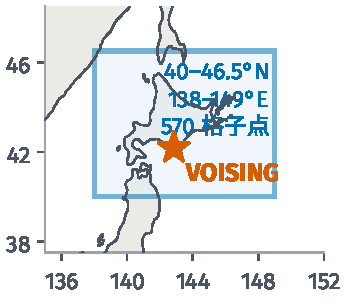
\includegraphics[width=\linewidth,height=70pt,keepaspectratio]{S_region_map.pdf}
    \end{column}
  \end{columns}
  \srcline{領域は北海道の箱 570 格子点、代表地点は VOISING。和歌山は比較用}
\end{frame}
